\section{List Mode Viewer}
This window is launched from within the main spectrum viewer application. Upon launching there are four individual graphs, seen in Figure \ref{fig:lmv}. This is used to split the list mode data acquired using the sync pulse and detector data. This will split that data relative to a sync pulse with an offset, with the data before the divider being referenced herein as region 1 and data after the divider as region 2.

\begin{figure}[h!]
	\centering
	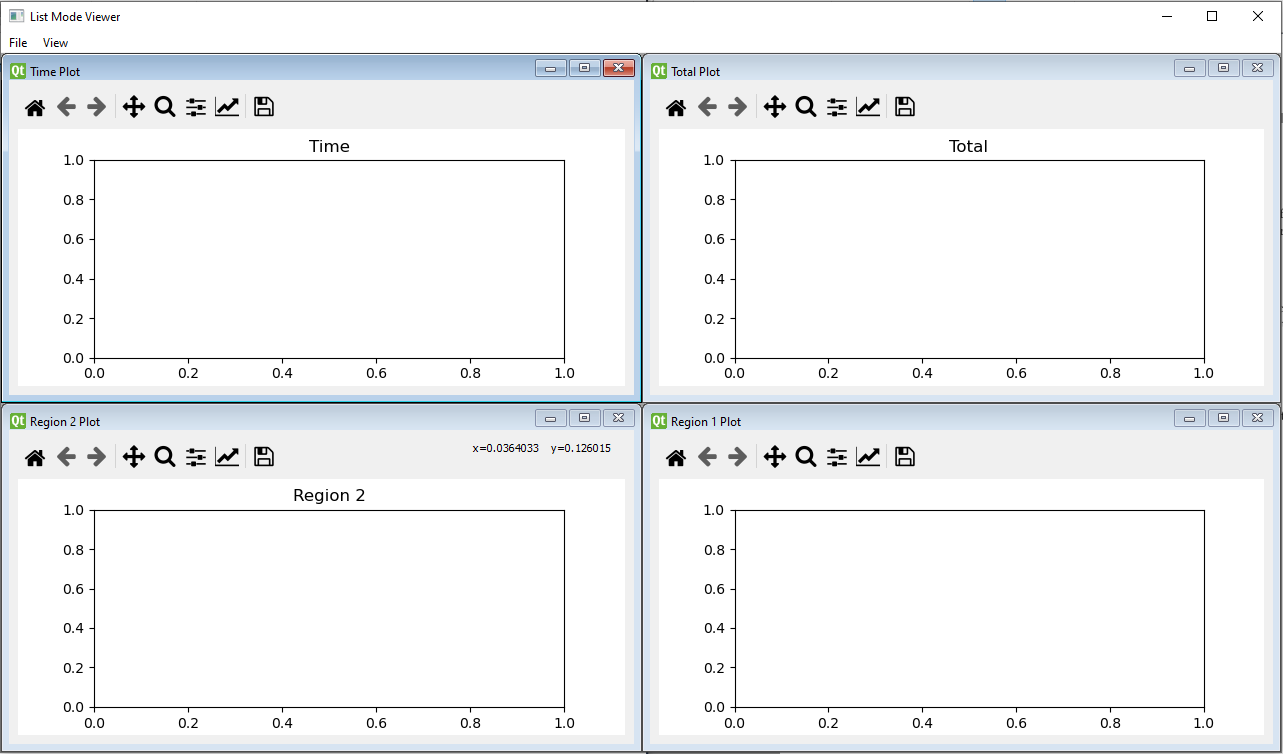
\includegraphics[width=\linewidth]{list_mode_viewer.png}
	\caption{Initial launching of list mode viewer}
	\label{fig:lmv}
\end{figure}

The top left graph will display the arrival of the pulse relative to the sync pulse. Top right will display the total spectrum as well as split data (region 1 \& 2). Bottom left will display only the region 2 spectrum, and the bottom right will display region 1 data.

\subsection{File Menu}
\subsubsection{Load New Data}
This launches the interface seen in Figure \ref{fig:new_loader}. The sync pulse and detector pulse are comma seperated files, corresponding to there respective files. It is expected that the comma seperated file will be in the form of having time, in nanoseconds, in the first column and a channel number being the second column. Once the files are loaded, the browse buttons with change to green. The final option is to add a calibration file, having been generated using the ``Calibrate Spectrum'' functionality. This is required to generate detection probability data.\\
\begin{figure}[h!]
	\centering
	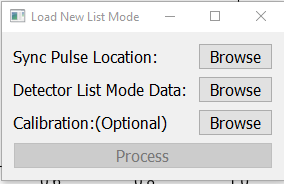
\includegraphics[width=0.5\linewidth]{load_new_viewer.png}
	\caption{List mode viewer data loader}
	\label{fig:new_loader}
\end{figure}

Once the appropriate files have been selected, the sync pulse and detector list mode data buttons will change to green. Additionally the process button will become enabled. Clicking the process button will initiate the process of reading the data in. The software will split the data into two regions by comparing the sync pulse arrival and the arrival of the lsit mode data. \textbf{This process can take several minutes dependent on file size and host computer.} The software will automatically calculate the frequency of the pulse arrival, but the software cannot determine the duty cylce of the pulse, as such, once the data has been imported and loaded, a new control panel be loaded, as seen in Figure \ref{fig:adjust_controls}. 

\begin{figure}[h!]
	\centering
	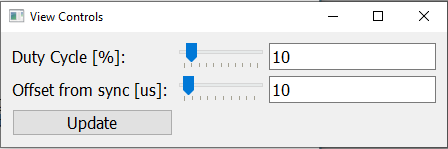
\includegraphics[width=0.5\linewidth]{control_panel.png}
	\caption{Control panel for adjusting duty cycle and offset times.}
	\label{fig:adjust_controls}
\end{figure}

This panel can be used to adjust the duty cycle, in percentage, and offset, in $\mu s$. The offset is the divider for region one and region two, while this is typically a positive integer, it is possible to adjust the slider bar negative. Both of these default to 10. It should be noted that adjustments must be made using the sldier bar for both values. Once a change has been made, the update button must be pressed, \textbf{again, this may take upwards of several minutes to process}. \\

As has been noted multiple times, this process is extremely memory intensive and time consuming. Use of a machine with limited memory is not advised, it is suggest that a minimum of 32GB of memory be installed in the machine. You can go online and download more memory if necessary.

\subsubsection{Save Spectrum}
This initiates a spectrum saving sequence. First is unsures the values in the controls window represent the data shown on the screen, this may take several minutes to validate. A pop up will appear to select the data to be saved, Region 1, Region 2, or Time Decay. Region 1 and Region2 will save a plain text file(.txt) having a single column of counts related to the channel. Time Decay will save either a plain text file (.txt) or comma-seperated file(.csv) having two columns, the first being time, in microseconds, the second being the number of counts accrued during that integration.
\subsubsection{Save ROI}
This initiates a raw data saving sequence. This will take the data from region 2 in a specified region of interest and save only these pulses to a seperate file, this is designed to be used for detection probability tools. The first windows explorer that will appear will ask for the location in which to save the comma seperated file. This file will have the energy, in MeV, followed by the time, in seconds for the two columns. If no calibration file was selected during loading of data, an additional file explorer will be displayed to select the desired calibration file. There will be two final pop-up windows to enter the region of interest. The data will be processed with no additional indications of success.

\subsection{View Menu}
The first two options in the view menu will shows the time adjustment tool and show all plots, respectively. The two remaining options investigate the consistency of sync pulse arrival and the arrival times of the region of interest pulses relative to the sync pulse. 

\subsubsection{Pulse Deviation}
This uses the sync pulse file to generate a arrival profile for the sync pulse. The file is parsed and the time delta between pulse arrival times is tabulated. The mean and standard deviation are calculated from this tabulation. A histogram is generated using the full featured plotting windows used for all other plots. The mean and standard deviation are displayed on the plot. 

\subsubsection{ROI Arrival Times}
The breakdown of when region of interest pulses arrive relative to the sync pulse is found. Using the two region dividers, three discrete regions can be defined in which the software will tabulate the number of pulses that occured through the entire accumulation. This generates a plot using the fully featured plotter and displays the breakdown of the three regions contribution to the total signal. \\

A save feature is incorporated so as to save the raw data generated from this. It will create a text file that has the percentage breakdown as the first line, followed by a two column format, time in microseconds, followed by associated counts. 

\section{Future Work}
As was stated in the introduction, this software is in beta testing, as such new features are continually being added and old features becoming more robust. New features that are currently being added include the ability to edit information inserted into the primary spectrum viewer and loading of different file formats into the spectrum viewer. 